\documentclass[17pt,mathserif]{beamer}
\usetheme{Singapore}
\usecolortheme{orchid}
\AtBeginSection{\frame{\sectionpage}}

\usepackage{listings}

\usepackage[english]{babel}
\usepackage[english]{isodate}
\cleanlookdateon

\newcommand{\oclass}[1]{\ensuremath{\mathtt{#1}}}
\newcommand{\osub}{\sqsubseteq}
\newcommand{\onsub}{\not\sqsubseteq}

\begin{document}

\title{Ontology Unit Testing}
\subtitle{Project Proposal}
\author{Ameerah Allie \and Kieren Davies}
\institute[UCT]{University of Cape Town}
\date{\printdate{2016-05-25}}
\titlepage

% \begin{frame}
%   \frametitle{Outline}
%   \tableofcontents
% \end{frame}

\section{Context}

\begin{frame}{Ontology engineering}
  \begin{itemize}
    \item Formal representation of knowledge
    \item Automatic reasoning
  \end{itemize}
  \centering
  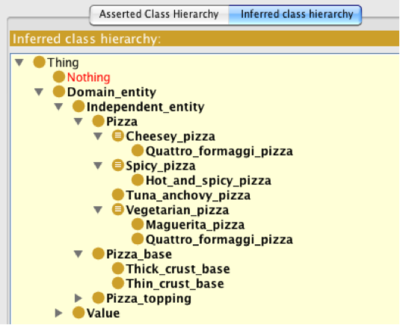
\includegraphics[width=0.5\textwidth]{pizza}
\end{frame}

\begin{frame}{Test-driven development}
  \begin{itemize}
    \item Successful in software engineering
    \item Ontology engineering less mature
    \begin{itemize}
      \item First test harnesses in 2015
      \item Reliant on reasoner
      \item Test-first
    \end{itemize}
  \end{itemize}
\end{frame}
\note{
  TDD:
  \begin{itemize}
    \item understandability
    \item reduced complexity
    \item code quality
    \item reliability: external tests passed
  \end{itemize}
}

\begin{frame}[t]{Why test?}
  \begin{align*}
    \oclass{Giraffe} &\osub \oclass{Herbivore} \\
    \oclass{Herbivore} &\osub \oclass{Mammal} \\
    \oclass{Mammal} &\osub \oclass{Animal}
  \end{align*}
\end{frame}

\begin{frame}[t]{Why test?}
  \begin{align*}
    \oclass{Giraffe} &\osub \oclass{Herbivore} \\
    \oclass{Herbivore} &\osub \oclass{Animal} \\
    \oclass{Mammal} &\osub \oclass{Animal} \\
    \\
    \oclass{Herbivore} &\onsub \oclass{Mammal}
  \end{align*}
\end{frame}
\note{
  Listing mammals misses giraffe
}

\begin{frame}{Related work}
  \begin{itemize}
    \item Vrande\v{c}i\'c and Gangemi
    \item Tawny-OWL (Warrender and Lord)
    \item SCONE (Neuhaus)
    \item TDDOnto ({\L}awrynowicz and Keet)
    \item OWL Reasoner Evaluation competition
  \end{itemize}
\end{frame}

\begin{frame}{Vrande\v{c}i\'c and Gangemi}
  \begin{align*}
    O &\models A_i^{+} \forall A_i^{+} \in T^{+} \\
    O &\not\models A_i^{-} \forall A_i^{-} \in T^{-}
  \end{align*}
\end{frame}
\note{
  No implementation
}

\begin{frame}[fragile]{Tawny-OWL}
  \begin{lstlisting}[language=Lisp,basicstyle=\normalsize\ttfamily]
(is
  (r/superclass?
    i/k46_XY
    n/MaleKaryotype))
  \end{lstlisting}
\end{frame}

\begin{frame}[fragile]{SCONE}
  \begin{lstlisting}[basicstyle=\footnotesize\ttfamily]
Scenario: Relative age between family members
  The parenthood relation entail an ordering of age.
  Given Chris is a parent of Dora.
  And Amy is a parent of Chris.
  And Amy is a parent of Berta.
  Then infer Chris is older than Dora.
  And infer Amy is older than Dora.
  And don’t infer Berta is older than Dora.
  And don’t infer Dora is older than Dora.
  \end{lstlisting}
\end{frame}

\begin{frame}{TDDOnto}
  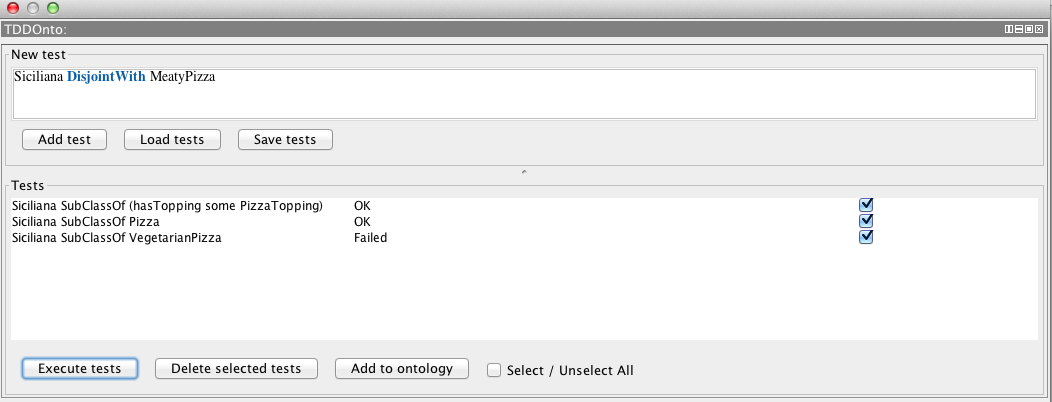
\includegraphics[width=\textwidth]{tddonto}
\end{frame}

\begin{frame}{OWL Reasoner Evaluation}
  \begin{itemize}
    \item Comparison of reasoner performance
    \item 14 reasoners tested
    \item Only OWL 2 DL and EL
  \end{itemize}
\end{frame}

\section{Problem}

\begin{frame}{Problem}
  \begin{itemize}
    \item Available tools don't support comprehensive tests
    \begin{itemize}
      \item No ABox or RBox
    \end{itemize}
    \item Not formally verified
    \begin{itemize}
      \item Only empirically
    \end{itemize}
    \item Performance of reasoner-based tests poorly understood
  \end{itemize}
\end{frame}

\begin{frame}{Problem statement: New tests}
  \begin{itemize}
    \item Previously described and implemented unit tests are not comprehensive
    \item No proof of correctness for any unit test algorithms
  \end{itemize}
\end{frame}

\begin{frame}{Research question: Benchmarking}
  \centering
  Which reasoner has the best performance on each of the unit test implementations?
\end{frame}

\begin{frame}{Aims}
  \begin{itemize}
    \item Improve ontology engineering process by
    \begin{itemize}
      \item defining and implementing more tests
      \item proving their correctness
      \item determining test performance of reasoners
    \end{itemize}
    \item Improve ontology quality, reduce complexity, improve understandability
    \item Encourage wider adoption of ontologies
  \end{itemize}
\end{frame}

\section{Methods}

\begin{frame}{New tests}
  \begin{enumerate}
    \item Create formal model
    \item Prove correctness of test from TDDOnto
    \item Describe new tests
    \item Prove correctness
    \item Implement
  \end{enumerate}
\end{frame}

\begin{frame}[allowframebreaks]{Benchmarking}
  \begin{enumerate}
    \item Gather ontologies
    \item Implement/obtain algorithm to generate unit tests
    \item Implement/obtain benchmark wrapper script
    \item Benchmarking one test type in one ontology
    \item Identify independent variables
    \item Modify script to do every combination of chosen variables
    \item Perform benchmarks, record results
    \item ANOVA on resulting data
  \end{enumerate}
\end{frame}
\note{
  \begin{itemize}
    \item First benchmark to check script and test generation
    \item Independent variables e.g.\ DL profile, ontology size
  \end{itemize}
}

\section{Outcomes}

\begin{frame}{Expected outcomes}
  \begin{itemize}
    \item Create suite of tests
    \begin{itemize}
      \item Approaching comprehensiveness
      \item Proven correct
    \end{itemize}
    \item Benchmark reasoners
    \begin{itemize}
      \item Statistically significant differences
      \item Better understand reasoner performance
      \item Inform choice of reasoners for future work
    \end{itemize}
  \end{itemize}
\end{frame}
\note{
  If not significant, still fine
}

\section{Plan}

\begin{frame}{Timeline}
  (Gantt chart)
\end{frame}

\begin{frame}{Risks}
  (Risk table)
\end{frame}

\begin{frame}{Ethical, legal, professional}
  \begin{itemize}
    \item Software licensing
    \begin{itemize}
      \item Prot\'eg\'e, TDDOnto, reasoners, scripts
      \item Our implementations
      \item Gathered ontologies
    \end{itemize}
    \item UCT IP policies
  \end{itemize}
\end{frame}

\end{document}
